\id{МРНТИ 65.09.30}{https://doi.org/10.58805/kazutb.v.2.27-1001}

\begin{articleheader}
\sectionwithauthors{А. Аблаева, Д.А. Тлевлесова, Б. Хамитова, Farah Saleena Taip, С.Т. Азимова, С. Бердіғалиұлы, Ф.А. Махмудов}{ОЦЕНКА ПИТАТЕЛЬНОЙ ЦЕННОСТИ И СТАБИЛЬНОСТИ РАСТИТЕЛЬНЫХ АНАЛОГОВ МОЛОКА}

{\bfseries
\textsuperscript{1}А. Аблаева\alink{https://orcid.org/0009-0007-1777-4001}\textsuperscript{\envelope },
\textsuperscript{2}Д.А. Тлевлесова\alink{https://orcid.org/0000-0002-5084-6587},
\textsuperscript{1}Б. Хамитова\alink{https://orcid.org/0000-0001-8377-3938},
\textsuperscript{3}Farah Saleena Taip\alink{https://orcid.org/0000-0002-2253-2302},
\textsuperscript{2}С.Т. Азимова\alink{https://orcid.org/0000-0002-8992-8889},
\textsuperscript{4}С. Бердіғалиұлы\alink{https://orcid.org/0000-0002-9776-831X},
\textsuperscript{5}Ф.А. Махмудов\alink{https://orcid.org/0000-0002-7791-1588}
}
\end{articleheader}

\begin{affiliation}
\textsuperscript{1}Южно-Казахстанский университет им.М.Ауезова, Шымкент, Казахстан,

\textsuperscript{2}Алматинский технологический университет,Алматы, Казахстан,

\textsuperscript{3}University Putra Malaysia, Putrajaya,~Malaysia,

\textsuperscript{4}Казахский университет технологий бизнеса им.К.Кулажанова, Астана, Казахстан,

\textsuperscript{5}Международный инженерно-технический университет, Алматы, Казахстан

\raggedright \textsuperscript{\envelope }Корреспондент-автор: ayzhanablayeva@gmail.com
\end{affiliation}

Лактозная непереносимость становится всё более распространённой
проблемой, что делает тему заменителей и аналогов молока актуальной. В
связи с этим активно развивается рынок альтернативных молочных
продуктов, включая растительное молоко, безлактозное молоко и продукты
на основе ферментированных растительных ингредиентов. В статье
представлены результаты комплексного анализа состава растительных
аналогов молока, включая молоко из пророщенного маша, зелёной гречки и
проса, с акцентом на содержание белков, жиров, углеводов, витаминов и
минералов. Проведённое сравнение с соевым и овсяным молоком позволило
выделить уникальные питательные свойства каждого типа молока. Были
исследованы и проанализированы методы обработки, такие как
ультразвуковая обработка, пастеризация и гомогенизация, которые
существенно повышают стабильность и продлевают срок хранения молока из
маша, гречки и проса. Сенсорные оценки показали, что молоко из
пророщенного маша и зелёной гречки обладает привлекательными
органолептическими характеристиками, включая ореховые и зерновые ноты,
что делает их особенно интересными для потребителей, ищущих разнообразие
вкусов. Особое внимание уделено обоснованию преимуществ этих
растительных аналогов, таких как высокое содержание магния,
антиоксидантов и клетчатки, что значительно повышает их ценность для
здоровья. На основе проведённого исследования даны рекомендации по
применению этих продуктов в различных категориях пищевой промышленности
и предложены направления для дальнейших научных исследований и
разработок.

{\bfseries Ключевые слова}: растительное молоко, пророщенный маш, зелёная
гречка, просо, ультразвуковая обработка, питательная ценность,
стабильность.

\begin{articleheader}
{\bfseries ӨСІМДІК ТЕКТЕС СҮТТІҢ ТАМАҚТЫҚ ҚҰНАРЛЫЛЫҒЫ МЕН ТҰРАҚТЫЛЫҒЫН БАҒАЛАУ}

{\bfseries
\textsuperscript{1}А.Аблаева\textsuperscript{\envelope },
\textsuperscript{2}Д.А. Тлевлесова,
\textsuperscript{1}Б. Хамитова,
\textsuperscript{3}Farah Saleena Taip,
\textsuperscript{2}С.Т. Азимова,
\textsuperscript{4}С. Бердіғалиұлы,
\textsuperscript{5}Ф.А. Махмудов
}
\end{articleheader}

\begin{affiliation}
\textsuperscript{1}М.Әуезов атындағы Оңтүстік Қазақстан университеті, Шымкент, Қазақстан,

\textsuperscript{2}Алматы технологиялық университеті, Алматы, Қазақстан,

\textsuperscript{3}University Putra Malaysia, Путраджая, Малайзия,

\textsuperscript{4}К.Кулажанов атындағы Қазақ бизнес және технология университеті, Астана, Қазақстан,

\textsuperscript{5}Халықаралық инженерлік-техникалық университеті, Алматы, Қазақстан,

e-mail: ayzhanablayeva@gmail.com
\end{affiliation}

Лактозаға төзбеушілік жиілеп бара жатқан өзекті мәселе болғандықтан,
сүттің алмастырғыштары мен өсімдік негізіндегі аналогтарын зерттеу
қажеттілігі артып келеді. Осыған байланысты өсімдік негізіндегі,
лактозасыз және ферменттелген өсімдік өнімдеріне негізделген сүттің
баламалары нарығы белсенді дамуда. Бұл мақалада маш, жасыл қарақұмық
және тары негізінде дайындалған өсімдік сүтінің құрамы -- ақуыздар,
майлар, көмірсулар, дәрумендер мен минералдар -- жан-жақты зерттеліп,
олардың соя және сұлы сүтімен салыстырмалы артықшылықтары көрсетілген.
Ультрадыбыстық өңдеу, пастерлеу және гомогенизация әдістері сүттің
тұрақтылығын арттыру және сақтау мерзімін ұзарту үшін қолданылды.
Сенсорлық бағалау нәтижесінде маш пен жасыл қарақұмықтан алынған сүттің
жаңғақ және дәнді дақылдарға тән дәмдік ерекшеліктері тұтынушылар үшін
тартымды екені анықталды. Сонымен қатар, магний, антиоксиданттар және
тағамдық талшықтардың жоғары мөлшері бұл өнімдердің адам денсаулығы үшін
құндылығын арттырады. Зерттеу нәтижелері өсімдік сүтінің түрлерін тамақ
өнеркәсібінде қолдану бойынша ұсыныстар жасауға және келешектегі ғылыми
зерттеулерге негіз бола алады.

{\bfseries Түйін сөздер:} өсімдік сүті, өнген маш, жасыл қарақұмық, тары,
ультрадыбыстық өңдеу, тағамдық құндылық, тұрақтылық.

\begin{articleheader}
{\bfseries EVALUATION OF THE NUTRITIONAL VALUE AND STABILITY OF PLANT-BASED
MILK ALTERNATIVES}

{\bfseries
\textsuperscript{1} A. Ablayeva\textsuperscript{\envelope },
\textsuperscript{2}D.A. Tlevlessova,
\textsuperscript{1}B. Khamitova,
\textsuperscript{3}Farah Saleena Taip,
\textsuperscript{2}S.T. Azimova,
\textsuperscript{4}S. Berdigaliuly,
\textsuperscript{5}F.A. Makhmudov
}
\end{articleheader}

\begin{affiliation}
\textsuperscript{1}M.Auezov South Kazakhstan University, Shymkent, Kazakhstan,

\textsuperscript{2}Almaty Technological University, Almaty, Kazakhstan,

\textsuperscript{3}University Putra Malaysia, Putrajaya, Malaysia,

\textsuperscript{4}Kazakh University of Business and Technology named after K. Kulazhanov, Astana, Kazakhstan,

\textsuperscript{5}International Engineering and Technical University, Almaty, Kazakhstan,

e-mail: ayzhanablayeva@gmail.com
\end{affiliation}

Lactose intolerance is becoming an increasingly common problem, making
the topic of milk substitutes and analogues highly relevant. As a
result, the market for alternative dairy products---including
plant-based, lactose-free, and fermented plant-based milk---is rapidly
growing. This study presents a comprehensive analysis of the composition
of plant-based milk made from sprouted mung beans, green buckwheat, and
millet, with a focus on protein, fat, carbohydrate, vitamin, and mineral
content. A comparison with soy and oat milk highlights the unique
nutritional properties of each milk type. Processing methods such as
ultrasonic treatment, pasteurization, and homogenization were
investigated to improve the stability and shelf life of the milk
alternatives. Sensory evaluations showed that milk from sprouted mung
beans and green buckwheat had appealing organoleptic characteristics,
including nutty and grainy notes, making them attractive to consumers
seeking variety in taste. Particular attention is given to their high
levels of magnesium, antioxidants, and dietary fiber, which
significantly enhance their health value. Based on the results, the
study offers recommendations for the use of these products in various
sectors of the food industry and outlines directions for further
scientific research and development.

{\bfseries Keywords:} plant-based milk, sprouted mung beans, green
buckwheat, millet, ultrasonic treatment, \\nutritional value, stability.

\begin{multicols}{2}
{\bfseries Введение.} Растительные молочко приобретают всё большую
популярность как альтернатива традиционному коровьему молоку. Основными
преимуществами являются их гипоаллергенность, отсутствие лактозы и
содержание различных полезных элементов. В данном исследовании был
проведен анализ элементного состава растительных аналогов молока из
зелёной гречки, пророщенного маша, проса и овса.

Для начала работы был проведен анализ актуальности данного исследования.
Проведен поиск научно-технической информации в наукометрических базах.
Результаты поиска по ключевому слову "растительное молоко" в базе данных
Scopus за период 2021-2024 годы представлены на рисунках 1 и 2.

Рисунок 1 отображает количество и распределение научных публикаций,
связанных с растительным молоком, в различных журналах и базах данных.
Период поиска охватывает последние четыре года, что позволяет
актуализировать информацию и исключить устаревшие данные.

Рисунок 2 представляет данные по публикациям, которые были опубликованы
исключительно в научных журналах и материалах конференций. Такой подход
позволяет сфокусироваться на наиболее релевантных и признанных научных
исследованиях в области растительных молочных аналогов.

\end{multicols}

\begin{figure}[H]
	\centering
	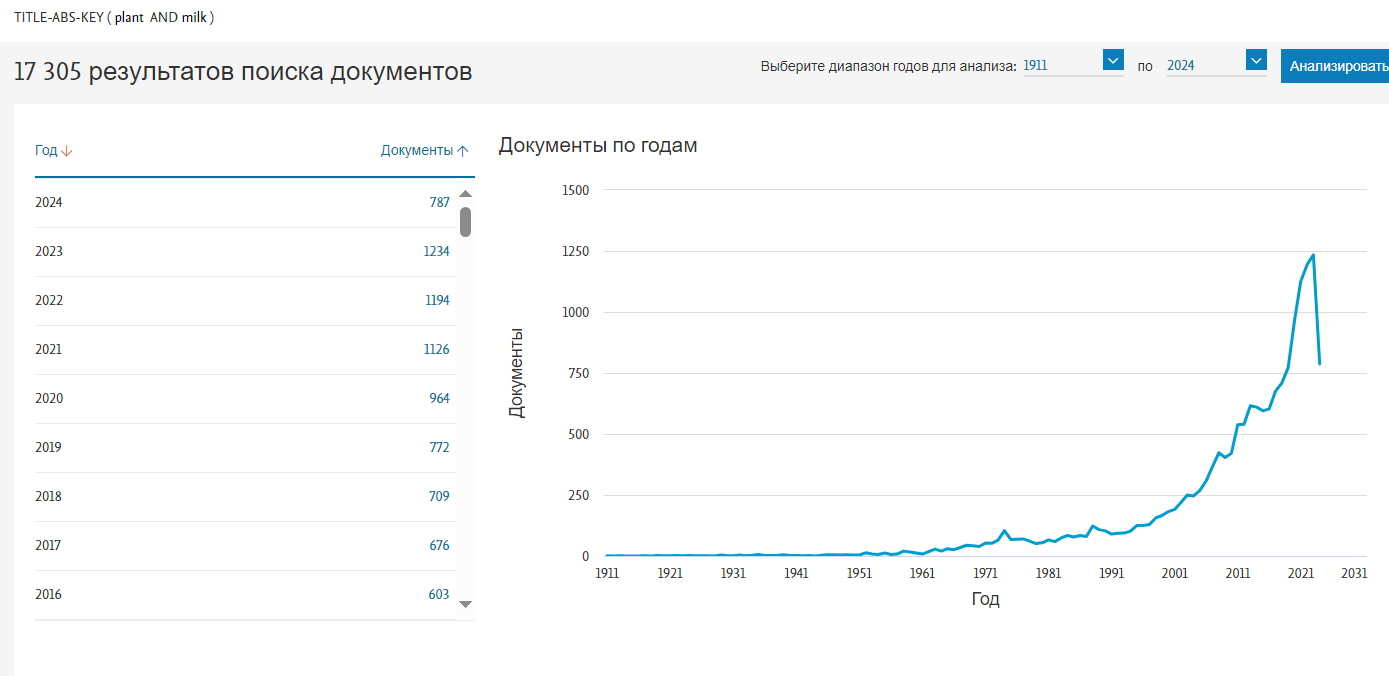
\includegraphics[width=0.75\textwidth]{media/pish/image47}
	\caption*{Рис.1 - поиск по ключевому слову растительное молоко в базе Скопус}
\end{figure}

\begin{figure}[H]
	\centering
	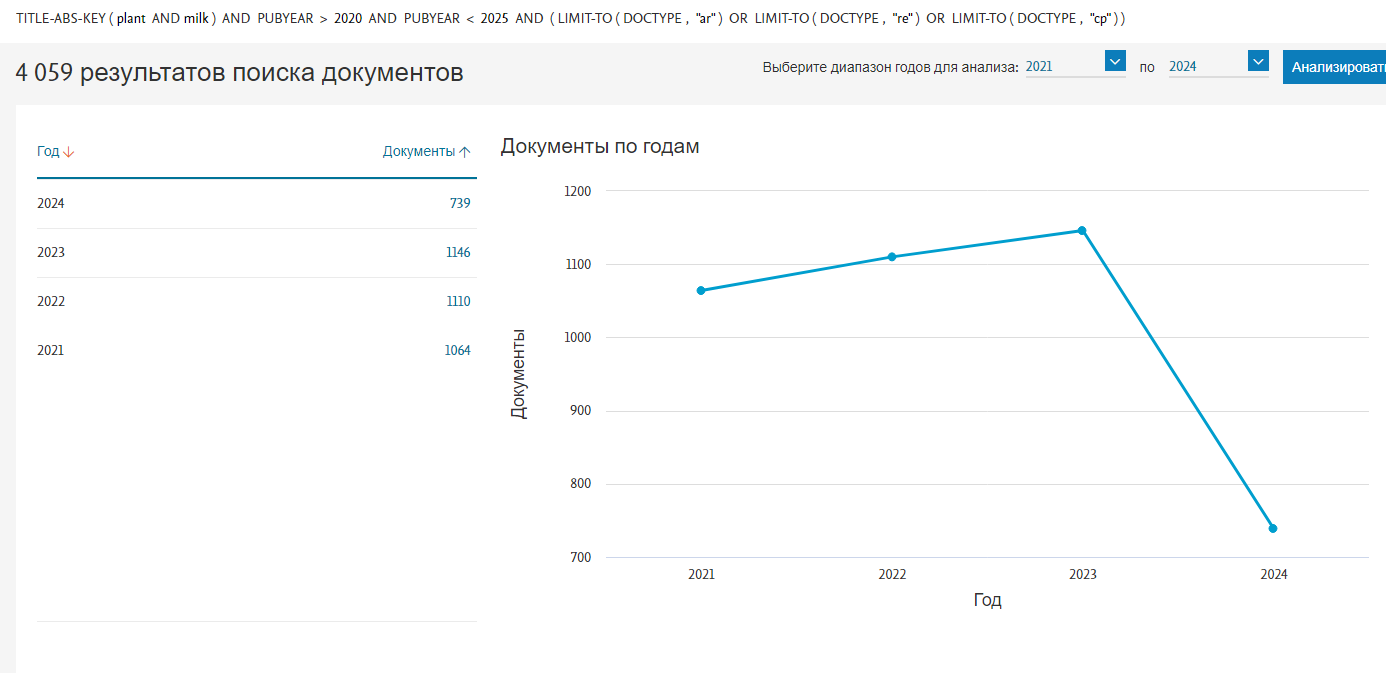
\includegraphics[width=0.75\textwidth]{media/pish/image48}
	\caption*{Рис.2 - поиск по ключевому слову растительное молоко тот же период только статьи в журналах и конференциях}
\end{figure}

\begin{multicols}{2}
В ходе данного исследования был проведен анализ текущих научных
публикаций, посвященных растительному молоку, с использованием базы
данных Scopus. В результате анализа выявлено, что за последние четыре
года интерес к теме растительных молочных продуктов значительно возрос.
Рисунки 1 и 2 показывают, что публикации, касающиеся растительного
молока, активно появляются как в научных журналах, так и на
конференциях, что подчеркивает актуальность темы и потребность в
дальнейшем изучении этого направления.

Разработка растительных аналогов молока является актуальной темой в
современной пищевой науке, поскольку растет потребность в продуктах,
которые могут заменить традиционное коровье молоко, особенно для людей
подверженных аллергии, непереносимостью лактозы или тех, кто следует
веганскому или вегетарианскому образу жизни.

Этот анализ подтверждает, что разработка растительных аналогов молока
продолжает оставаться важной и востребованной областью исследования,
особенно в контексте растущего спроса на альтернативы традиционному
коровьему молоку.

Одним из ключевых аспектов разработки растительных молочных аналогов
является обеспечение их питательной ценности, сопоставимой с коровьим
молоком. Соевое молоко, например, известно своим высоким содержанием
белка, который составляет около 3,4 г на 100 мл, что делает его одним из
наиболее питательных растительных аналогов {[}1, 2{]}.

Овсяное молоко, с другой стороны, содержит больше углеводов, что делает
его популярным выбором среди людей, ищущих источник энергии с низким
содержанием жиров. В то же время такие аналоги, как молоко из
пророщенного маша, зелёной гречки и проса, предлагают уникальные
питательные профили, которые делают их ценными дополнениями к рациону
{[}1{]}. Например, маш и гречка богаты магнием и антиоксидантами, что
способствует улучшению здоровья сердечно-сосудистой системы и снижению
уровня воспалений.

Растительные аналоги молока, как правило, подвержены фазовой сепарации и
микробной порче, что ограничивает их срок хранения. Однако современные
технологии, такие как ультразвуковая обработка, пастеризация и
добавление стабилизаторов, позволяют значительно улучшить стабильность и
продлить срок хранения этих продуктов {[}3{]}. Например, исследования
показали, что ультразвуковая обработка может уменьшить размер частиц,
улучшая текстуру и предотвращая разделение фаз в соевом и овсяном
молоке.

Органолептические характеристики, такие как вкус, текстура и аромат,
являются важными факторами, влияющими на принятие потребителями
растительных молочных аналогов. Соевое молоко, несмотря на свои
питательные преимущества, может иметь специфический вкус, который не
всем нравится, в то время как миндальное молоко часто предпочитается за
его мягкий вкус и легкую текстуру {[}4{]}. Молоко из пророщенного маша и
гречки обладает уникальными вкусовыми характеристиками, такими как
ореховые и зерновые нотки, что делает их интересными для тех, кто ищет
разнообразие вкусов в своем рационе.

Растительные молочные аналоги также предлагают различные преимущества
для здоровья, включая гипоаллергенные свойства, отсутствие лактозы и
наличие полезных фитонутриентов. Молоко из маша и гречки, например,
богато антиоксидантами и полифенолами, которые могут способствовать
снижению риска сердечно-сосудистых заболеваний и улучшению общего
состояния здоровья {[}5-11{]}.

Так же были исследованы изменения в показателях качества коммерческих
напитков из миндаля и овса при микробиальной ферментации. Их работа
показала, что ферментация улучшает органолептические характеристики и
питательную ценность растительных напитков. Увеличилось содержание
полезных бактерий, что делает такие напитки функциональными продуктами
для поддержания здоровья желудочно-кишечного тракта {[}12{]}. Была
проведена питательная оценка соевого молока и его продуктов.
Исследование показало, что регулярное потребление этих продуктов
способствует улучшению глюколипидного профиля крови, включая снижение
уровня холестерина и триглицеридов, что подтверждает их пользу для
сердечно-сосудистой системы {[}13{]}. Использование пророщенных соевых
бобов улучшает функциональные свойства соевого молока, включая его
текстуру, вкусовые характеристики и стабильность. Пророщенные бобы
обогащают молоко антиоксидантами и аминокислотами, что делает его более
питательным {[}14{]}. Использование атмосферной нетепловой плазменной
системы для микробной деконтаминации овсяного молока оказалось
эффективным для снижения микробной нагрузки без изменения
физико-химических свойств продукта, что позволяет продлить его срок
хранения {[}15{]}. Исследование {[}16{]} показало, что правильный выбор
модели фильтрации влияет на стабильность продукта и позволяет снизить
уровень нежелательных примесей, что особенно важно для крупномасштабного
производства растительных напитков.

Ключевые аспекты стабильности растительных молочных аналогов были
исследованы в обзоре \emph{Stability Aspects of Non-Dairy Milk
Alternatives} (IntechOpen). Авторы отметили, что использование
стабилизаторов, ультразвуковой обработки и ферментации значительно
снижает фазовую сепарацию и улучшает текстуру напитков {[}3{]}.

Анализ статьи \emph{Plant-Based Milk Substitutes: Factors to Lead to Its
Use and Benefits to Human Health} (IntechOpen) показал, что растительные
аналоги молока являются не только альтернативой для людей с
непереносимостью лактозы, но и источником необходимых нутриентов, таких
как кальций, белки и витамины. Однако их питательная ценность сильно
зависит от используемого сырья и технологий обработки. Производство
растительных молочных аналогов, как правило, требует меньше ресурсов и
оказывает меньшее воздействие на окружающую среду по сравнению с
производством коровьего молока. Например, выращивание сои, овса и
некоторых зерновых культур требует меньше воды и земли, что делает эти
продукты более устойчивыми и экологичными {[}17{]}. Кроме того,
растительное молоко является важным компонентом веганского и
вегетарианского образа жизни, что способствует снижению использования
продуктов животного происхождения и уменьшению углеродного следа.

В работе \emph{A Comparative Analysis of Plant-Based Milk Alternatives}
(2022) проведён сравнительный анализ растительных молочных аналогов по
их составу, органолептическим характеристикам и питательной ценности.
Миндальное молоко выделяется мягким вкусом, овсяное --- высокой
концентрацией углеводов, а соевое --- богатством белков. Несмотря на
различия, все виды напитков получили положительную оценку за
экологичность и низкий углеродный след {[}18{]}.

В обзоре литературы было показано, что разработка растительных аналогов
молока, таких как соевое, овсяное, миндальное, а также молоко из
пророщенного маша, зелёной гречки и проса, имеет множество преимуществ.
Эти продукты не только обеспечивают питательные вещества, необходимые
для поддержания здоровья, но и предлагают разнообразие вкусов и текстур,
которые могут удовлетворить различные предпочтения потребителей.
Современные технологии обработки позволяют улучшить стабильность и срок
хранения растительных молочных аналогов, делая их более удобными и
доступными для широкого круга потребителей. Экологические и этические
аспекты также играют важную роль в популяризации этих продуктов.

Таким образом, растительные аналоги молока представляют собой
перспективную альтернативу традиционному молоку, удовлетворяющую
потребности как в питательных веществах, так и в улучшении устойчивости
пищевых систем.

Цель данной статьи заключается в обосновании разработки и оценки
растительных аналогов молока, таких как молоко из пророщенного маша,
зелёной гречки и проса, с точки зрения их питательной ценности,
стабильности, органолептических характеристик и пользы для здоровья.
Особое внимание уделяется сравнению с традиционными аналогами, такими
как соевое и овсяное молоко, а также определению их места в рационе
современного потребителя.

Гипотеза исследования заключается в том, что молоко из пророщенного
маша, зелёной гречки и проса может не только успешно конкурировать с
традиционными растительными аналогами, такими как соевое и овсяное
молоко, но и предложить уникальные преимущества, благодаря своим
специфическим питательным и функциональным свойствам.

Новизна статьи состоит в комплексном подходе к оценке растительных
молочных аналогов из менее распространённых злаков и бобовых, таких как
маш, гречка и просо. В отличие от большинства существующих исследований,
акцент сделан на уникальных питательных свойствах, органолептических
характеристиках и технологических аспектах обработки этих продуктов, что
позволяет предложить новые возможности для их использования в пищевой
промышленности.

{\bfseries Задачи.} Для достижения поставленной цели и проверки гипотезы в
статье решаются следующие задачи:

- провести сравнительный анализ питательной ценности растительных
аналогов молока, включая содержание белков, жиров, углеводов, витаминов
и минералов;

- оценить стабильность растительных молочных продуктов при хранении,
используя современные методы обработки и консервации;

- исследовать органолептические характеристики (вкус, текстура, аромат)
различных типов растительного молока и определить их потребительскую
привлекательность;

- обосновать преимущества использования менее распространённых злаков и
бобовых (маш, гречка, просо) в качестве основы для растительных молочных
аналогов с точки зрения их пользы для здоровья и экологической
устойчивости.

- разработать рекомендации по использованию растительных молочных
аналогов в различных категориях пищевой продукции, учитывая их
специфические свойства и предпочтения потребителей.

{\bfseries Материалы и методы.} \emph{Подготовка растительных молочных
аналогов}: Суспензии из каждого вида сырья готовились путём
измельчения зёрен с добавлением воды в соотношении 1:3. Жидкость
фильтровалась для отделения твёрдых частиц, а затем подвергалась
ультразвуковой обработке для повышения стабильности.
\end{multicols}

\tcap{Таблица 1 - Минеральный и витаминный состав растительного молока из маша, гречки и проса}
\begin{longtblr}[
  label = none,
  entry = none,
]{
  width = \linewidth,
  colspec = {Q[212]Q[331]Q[202]Q[194]},
  cells = {c},
  hlines,
  vlines,
}
\textbf{Показатель} & \textbf{Молоко из маша}      & \textbf{Молоко из гречки} & \textbf{Молоко из проса} \\
Калий (K)           & 15.95\%                      & 29.29\%                   & 16.35\%                  \\
Фосфор (P)          & 15.84\%                      & 7.18\%                    & 10.43\%                  \\
Магний (Mg)         & 5.21\%                       & 4.24\%                    & 3.64\%                   \\
Кальций (Ca)        & 1.14\%                       & 3.62\%                    & 1.21\%                   \\
Железо (Fe)         & 0.32\%                       & —                         & —                        \\
Витамин C           & Высокий (после проращивания) & Умеренный                 & —                        \\
Витамины группы B   & B1, B2                       & B1, B2, B3                & B3                       \\
Витамин E           & Следы                        & Присутствует              & Присутствует             \\
Рутин (витамин P)   & —                            & Присутствует              & —                        \\
β-каротин           & —                            & —                         & Присутствует             
\end{longtblr}

\begin{multicols}{2}
{\bfseries Химический анализ состава:} Для анализа элементного состава
использовался спектрометрический метод, проводившийся в ИРЛИП "К и Б М"
ЮКУ им. М. Ауезова. Весовой процент каждого элемента (C, O, Na, Mg, P,
S, K, Ca и др.) был рассчитан для всех образцов (см. данные). Анализ
каждого образца проводился с целью определения процентного содержания
элементов, таких как углерод (C), кислород (O), натрий (Na), магний
(Mg), алюминий (Al), кремний (Si), фосфор (P), сера (S), хлор (Cl),
калий (K), кальций (Ca) и железо (Fe). Применение спектрального анализа
позволило выявить особенности химического состава растительного молока,
полученного из разных источников, что может оказывать влияние на его
питательную ценность и функциональные свойства.

Измерение pH и вязкости растительного молока позволяет оценить его
стабильность и пригодность к хранению. Эти параметры часто измеряются с
использованием рН-метров и вискозиметров {[}3{]}.

Изучение различных технологических процессов, таких как ультразвуковая
обработка, гомогенизация, пастеризация и ультравысокое давление. Эти
методы применяются для повышения стабильности растительного молока и
продления сроков его хранения {[}1{]}. Анализировали, как различные
методы обработки влияют на питательные характеристики и сенсорные
свойства растительного молока, включая сохранение витаминов и минералов,
а также предотвращение разделения фаз {[}3{]}. Ультразвуковой аппарат
\emph{Sonics VCX-500} (мощность 400 Вт, частота 20 кГц) использовался
для стабилизации смеси.

Для химического анализа состава использовали \emph{Спектрометр Thermo
Nicolet FTIR} с целью определения содержания элементов.

{\bfseries Результаты и обсуждение.}

1. \emph{{\bfseries Нутриентный анализ.}} Пищевая ценность растительных
молочных напитков в
значительной степени определяется их витаминно-минеральным составом,
который зависит как от исходного растительного сырья, так и от метода
обработки.

Элементы минерального состава были определены методом электронно-лучевой
спектроскопии (ИРЛИП ЮКУ им. М. Ауезова). Эти данные приведены в Таблице

Результаты (табл.1) показывают, что каждый вид растительного молока
имеет специфический витаминно-минеральный профиль, отражающий
биохимические особенности соответствующего сырья:

- молоко из пророщенного маша выделяется высоким содержанием фосфора и
калия,
а также богатым комплексом водорастворимых витаминов (C и группы B), что
делает его особенно полезным для поддержания метаболизма и
восстановления после физических нагрузок;

- гречневое молоко является лидером по содержанию калия и обладает
антиоксидантными свойствами за счёт наличия рутина и витамина E. Оно
также содержит значимые количества магния и витаминов B-комплекса,
способствуя улучшению сосудистого и нервного здоровья;

- молоко из проса обладает сбалансированным минеральным составом, с
наличием β-каротина, что делает его перспективным средством для
профилактики дефицита витамина A и поддержания зрения. Также в нём
выявлено достаточное содержание фосфора и витамина B3.
Таким образом, все три напитка могут быть отнесены к функциональным
продуктам питания. В зависимости от состава, они могут быть
рекомендованы для включения в рацион определённых групп населения:
детей, спортсменов, пожилых людей, а также лиц с нарушениями углеводного
обмена и сосудистыми заболеваниями.

{\bfseries Молочко из зеленой гречки.} На рисунке 3 представлена
визуализация элементного состава растительного молока, приготовленного
из зелёной гречки. Данные спектрального анализа позволяют выделить
ключевые макро- и микроэлементы, обеспечивающие высокую питательную
ценность продукта.
\end{multicols}

\begin{figure}[H]
	\centering
	\begin{subfigure}{0.4\textwidth}
		\centering
		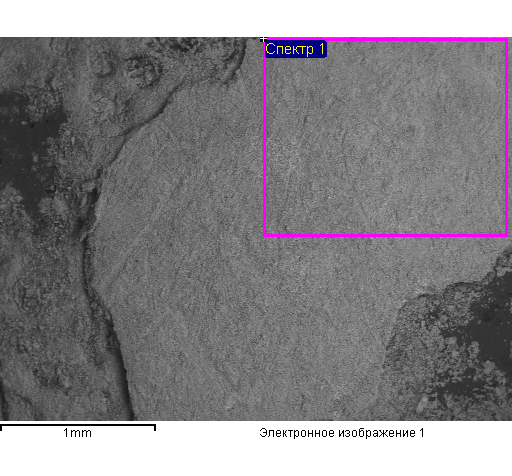
\includegraphics[height=5cm]{media/pish/image49}
	\end{subfigure}
	\hfill
	\begin{subfigure}{0.55\textwidth}
		\centering
		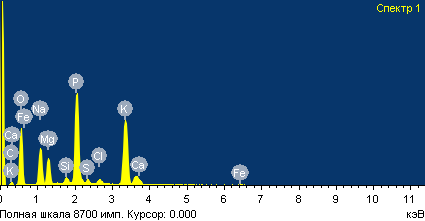
\includegraphics[height=5cm]{media/pish/image50}
	\end{subfigure}
    \caption*{Рис.3 - Молочко зелёной гречки}
\end{figure}


\begin{multicols}{2}
Состав включает в себя значительное количество кислорода (36,87\%) и
калия (29,29\%), а также присутствие таких элементов, как магний
(4,24\%) и фосфор (7,18\%). Эти данные свидетельствуют о высоком
содержании питательных веществ, особенно калия, что делает этот вид
молочка полезным для поддержания электролитного баланса в организме.

{\bfseries Молочко из пророщенного маша.} На рисунке 4 приведён элементный
состав молочка, приготовленного из пророщенного маша. Полученные данные
демонстрируют высокое содержание кислорода, фосфора и натрия, что
указывает на значительный функциональный потенциал данного напитка в
рационе питания.
\end{multicols}

\begin{figure}[H]
	\centering
	\begin{subfigure}{0.4\textwidth}
		\centering
		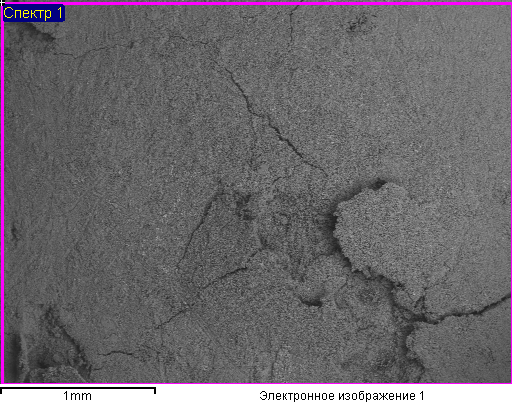
\includegraphics[height=5cm]{media/pish/image51}
	\end{subfigure}
	\hfill
	\begin{subfigure}{0.55\textwidth}
		\centering
		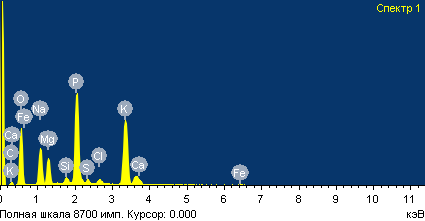
\includegraphics[height=5cm]{media/pish/image50}
	\end{subfigure}
	\caption*{Рис.4 - Молочко из пророщенного маша}
\end{figure}

\begin{figure}[H]
	\centering
	\begin{subfigure}{0.4\textwidth}
		\centering
		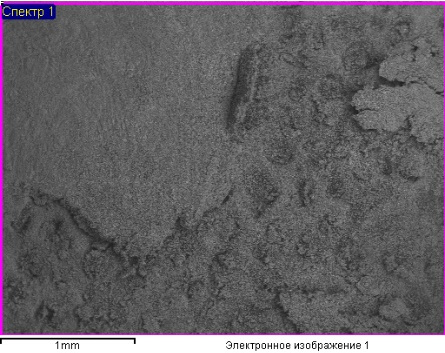
\includegraphics[height=5cm]{media/pish/image52}
	\end{subfigure}
	\hfill
	\begin{subfigure}{0.55\textwidth}
		\centering
		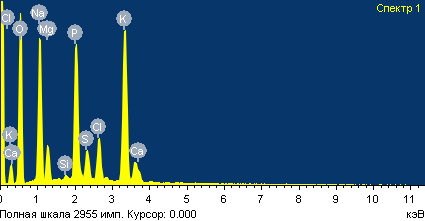
\includegraphics[height=5cm]{media/pish/image53}
	\end{subfigure}
	\caption*{Рис.5 - Молочко из проса}
\end{figure}

\begin{multicols}{2}
Данный образец отличается высоким содержанием кислорода (39,43\%) и фосфора
(15,84\%), а также значительным содержанием натрия (10,00\%). Высокий
уровень фосфора указывает на потенциал этого молочка в укреплении
костной ткани и зубов.

{\bfseries Молочко из проса.} На рисунке 5 представлен элементный состав
молочка из проса. Образец отличается высоким содержанием кислорода и
натрия, а также значительным уровнем фосфора и калия, что
свидетельствует о его питательной ценности и возможной антиоксидантной
активности.

Молочко из проса содержит наибольший процент кислорода (44,65\%) и
натрия (17,14\%), что может указывать на его высокие окислительные
свойства. Наличие фосфора (10,43\%) и калия (16,35\%) также выделяет
этот продукт среди остальных по своим питательным характеристикам.

{\bfseries Молочко из овса.} Этот образец характеризуется высоким
содержанием кислорода (38,62\%) и калия (22,96\%), а также магния
(8,83\%) и фосфора (18,30\%). Учитывая такие показатели, овсяное молочко
можно рассматривать как богатый источник магния, который играет важную
роль в функционировании нервной системы и мышц.
\end{multicols}

\begin{figure}[H]
	\centering
	\begin{subfigure}{0.4\textwidth}
		\centering
		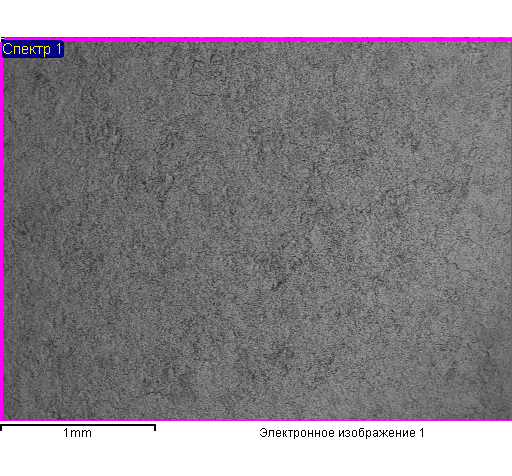
\includegraphics[height=5cm]{media/pish/image55}
	\end{subfigure}
	\hfill
	\begin{subfigure}{0.55\textwidth}
		\centering
		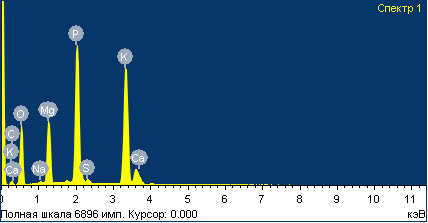
\includegraphics[height=5cm]{media/pish/image56}
	\end{subfigure}
	\caption*{Рис.6 - Молочко из овса}
\end{figure}

\begin{multicols}{2}
Анализ результатов показал что: Содержание кислорода (O) во всех
образцах варьируется, но наибольшее содержание наблюдается в молочке из
проса (44.65\%), а наименьшее --- в молочке из зеленой гречки (36.87\%).

Содержание натрия (Na) значительно варьируется, с наибольшим процентом в
молочке из проса (17.14\%) и наименьшим в молочке из овса (0.46\%).

Калий (K) наиболее высок в молочке из зеленой гречки (29.29\%) и овса
(22.96\%), что делает эти молочки хорошими источниками этого элемента.

Магний (Mg) наибольший процент содержится в молочке из овса (8.83\%) и
пророщенного маша (5.21\%).

Фосфор (P) наиболее высок в молочке из овса (18.30\%) и пророщенного
маша (15.84\%).

Кальций (Ca) содержится в наибольшем количестве в молочке из зеленой
гречки (3.62\%) и наименьшее в молочке из маша (1.14\%).

На основе приведенных данных можно заключить, что каждое из приведенных
видов растительного молочка имеет свои уникальные свойства. Молочко
зелёной гречки и овса отличаются высоким содержанием калия, что делает
их полезными для сердечно-сосудистой системы. В то же время молочко из
пророщенного маша выделяется высоким уровнем фосфора, а молочко из проса
содержит наибольшее количество натрия.
\end{multicols}

\tcap{Таблица 2 - Сравнительный анализ макроэлементов и жирных кислот в различных типах растительного молока}
\begin{longtblr}[
  label = none,
  entry = none,
]{
  width = \linewidth,
  colspec = {Q[171]Q[156]Q[154]Q[187]Q[271]},
  cells = {c},
  hlines,
  vlines,
}
\textbf{Тип молока} & \textbf{Белок (г/100 мл)} & \textbf{Жиры (г/100 мл)} & \textbf{Углеводы (г/100 мл)} & \textbf{Основные жирные кислоты}                        \\
Соевое              & 3.4                       & 2.0                      & 4.5                          & {Линолевая кислота (C18:2),\\Олеиновая кислота (C18:1)} \\
Миндальное          & 0.4                       & 2.8                      & 0.2                          & Линолевая кислота (C18:2)                               \\
Овсяное             & 1.0                       & 1.5                      & 8.0                          & Линолевая кислота (C18:2)                               \\
Рисовое             & 0.1                       & 1.0                      & 9.0                          & Линолевая кислота (C18:2)                               \\
Пророщенный маш     & 1.1                       & 0.3                      & 7.5                          & Линолевая кислота (C18:2)                               \\
Зелёная гречка      & 1.2                       & 0.5                      & 6.8                          & Линоленовая кислота (C18:3)                             \\
Просо               & 0.9                       & 0.7                      & 9.2                          & Пальмитиновая кислота (C16:0)                           
\end{longtblr}

\begin{multicols}{2}
2. \emph{{\bfseries Физико-химический анализ.}} Таблица 2 представляет
сравнительный анализ макроэлементов и жирных кислот в различных типах
растительного молока.

\emph{Из таблицы 2 видно}, что соевое молоко обладает самым высоким
содержанием белка, тогда как рисовое и просо содержат наибольшее
количество углеводов. Пророщенный маш и зелёная гречка демонстрируют
сбалансированный состав с умеренным содержанием белков и углеводов.

{\bfseries \emph{pH и вязкость}.} Таблица 3 - иллюстрирует показатели pH и
вязкости различных типов растительного молока при 25°C
\end{multicols}

\tcap{Таблица 3 - pH и вязкость различных типов растительного молока при 25°C}
\begin{longtblr}[
  label = none,
  entry = none,
]{
  cells = {c},
  hlines,
  vlines,
}
\textbf{Тип молока} & \textbf{pH} & \textbf{Вязкость (mPa·s)} \\
Соевое              & 7.0         & 10.5                      \\
Миндальное          & 6.8         & 3.5                       \\
Овсяное             & 6.5         & 6.0                       \\
Рисовое             & 6.0         & 2.8                       \\
Пророщенный маш     & 6.2         & 4.2                       \\
Зелёная гречка      & 6.7         & 5.0                       \\
Просо               & 6.4         & 5.5                       
\end{longtblr}

\begin{multicols}{2}
\emph{Согласно таблице 2}, соевое молоко имеет наиболее нейтральный pH и
наибольшую вязкость, что может влиять на его текстуру и стабильность.
Пророщенный маш и зелёная гречка демонстрируют близкие к нейтральному
значения pH, обеспечивая приятный вкус и стабильность продукта.

{\bfseries 3. \emph{Органолептический анализ}}

Сравнительная органолептическая оценка растительных молочных аналогов по
критериям вкуса, аромата и текстуры. В исследовании представлены
наиболее популярные образцы на основе сои, миндаля, овса, а также
альтернативные напитки из пророщенного маша, зелёной гречки и проса.
Каждому параметру была присвоена оценка по 9-балльной шкале
экспертами-дегустаторами.

На основании приведённых данных видно, что {\bfseries миндальное молоко
лидирует по вкусу,} в то время как {\bfseries продукты из проса и зелёной
гречки демонстрируют наилучшую текстуру.} Интересно отметить, что
{\bfseries молоко из пророщенного маша} имеет схожие показатели с
традиционными видами и может служить полноценной альтернативой, особенно
по аромату. Это подтверждает перспективность менее распространённых
злаков и бобовых в разработке органолептически привлекательных
растительных напитков.
\end{multicols}

\begin{figure}[H]
	\centering
	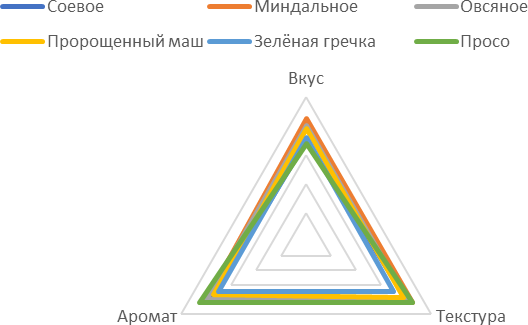
\includegraphics[width=0.5\textwidth]{media/pish/image57}
	\caption*{Рис.7 - Сравнительная органолептическая оценка растительных молочных аналогов по критериям вкуса, аромата и текстуры}
\end{figure}

{\bfseries 4. \emph{Микробиологический анализ}}

Таблица 4 демонстрирует микробную нагрузку в различных типах
растительного молока.

\tcap{Таблица 4 - Микробная нагрузка в различных типах растительного молока (CFU/мл)}
\begin{longtblr}[
  label = none,
  entry = none,
]{
  cells = {c},
  hlines,
  vlines,
}
\textbf{Тип молока} & \textbf{Общая микробная нагрузка} & \textbf{Наличие патогенов (CFU/мл)} \\
Соевое              & 100                               & Отсутствуют                         \\
Миндальное          & 100                               & Отсутствуют                         \\
Овсяное             & 500                               & Отсутствуют                         \\
Рисовое             & 500                               & Отсутствуют                         \\
Пророщенный маш     & 200                               & Отсутствуют                         \\
Зелёная гречка      & 150                               & Отсутствуют                         \\
Просо               & 300                               & Отсутствуют                         
\end{longtblr}

\begin{multicols}{2}
\emph{Таблица 4 показывает}, что все образцы растительного молока имеют
низкую микробную нагрузку и отсутствие патогенов, что свидетельствует о
их безопасности при правильной обработке и хранении.

{\bfseries 5. \emph{Технологический анализ.}} Стабильность растительных
молочных напитков является ключевым показателем их технологической
пригодности и потребительской ценности.

Учитывая особенности сырья - пророщенного маша, зелёной гречки и проса -
для обеспечения микробиологической безопасности, сохранения питательных
веществ и улучшения органолептических характеристик были отобраны три
основных метода обработки: мягкая термообработка (бланширование),
гомогенизация и пастеризация.

Выбор этих методов основан на их широком применении в технологии
растительных напитков, а также на научных публикациях, подтверждающих их
эффективность в стабилизации суспензий, инактивации патогенной
микрофлоры и снижении содержания антинутриентов. При этом каждый тип
сырья требует индивидуального подхода, так как избыточная обработка
может привести к потере функциональных свойств, а недостаточная - к
нестабильности продукта при хранении.

В таблице 5 представлены оптимальные комбинации методов обработки,
отобранные с учётом характеристик каждого вида растительного молока:
\end{multicols}

\tcap{Таблица 5 - Влияние методов обработки на стабильность растительного молока}
\begin{longtblr}[
  label = none,
  entry = none,
]{
  width = \linewidth,
  colspec = {Q[238]Q[150]Q[200]Q[371]},
  row{1} = {c},
  cell{2}{1} = {c},
  cell{2}{2} = {c},
  cell{2}{3} = {c},
  cell{3}{1} = {c},
  cell{3}{2} = {c},
  cell{3}{3} = {c},
  cell{4}{1} = {c},
  cell{4}{2} = {c},
  cell{4}{3} = {c},
  hlines,
  vlines,
}
\textbf{Метод обработки}            & \textbf{Тип молока} & \textbf{Стабильность (дни хранения)} & \textbf{Заметки}                                         \\
Мягкая термообработка и измельчение & Пророщенный маш     & 7                                    & Бланширование снижает антинутриенты и микробную нагрузку \\
Гомогенизация и пастеризация        & Зелёная гречка      & 10                                   & Улучшение текстуры, вкуса и однородности                 \\
Термическая обработка               & Просо               & 8                                    & Снижение микробной нагрузки, повышение сроков хранения   
\end{longtblr}

\begin{multicols}{2}
Пророщенный маш содержит активные ферменты, аминокислоты и
чувствительные биоактивные вещества. Поэтому основным методом выбрана
мягкая термообработка --- бланширование при 70-80\,°C позволяет
обеспечить микробиологическую безопасность и уменьшить содержание
ингибиторов ферментов, сохранив биологическую активность.

Для зелёной гречки была применена комбинация гомогенизации и
пастеризации, что обусловлено необходимостью стабилизировать текстуру,
улучшить вкус и продлить срок хранения. Гречневое молоко склонно к
окислительным процессам, поэтому пастеризация также выполняет
антиоксидантную роль.

Просо, благодаря своей волокнистой структуре и плотной текстуре, требует
умеренной термической обработки, что обеспечивает стабильность и
предотвращает разделение фаз без необходимости в более сложной
обработке.

Таким образом, оптимизация обработки каждого типа растительного молока
позволила достичь баланса между стабильностью, безопасностью и
сохранением полезных свойств. Эти подходы могут быть рекомендованы для
промышленного производства инновационных функциональных напитков.

\emph{{\bfseries Рекомендации:}}

- соевое молоко использовать для обогащения белком спортивных напитков и
функциональных коктейлей;

- миндальное молоко предлагать для низкокалорийных десертов и напитков;

- овсяное и рисовое молоко использовать как основу для напитков с
высокой углеводной ценностью (энергетики);

- молоко из пророщенного маша и зелёной гречки включить в линейки
продуктов для специализированных диет;

- рекомендовать комбинированные методы обработки (гомогенизация,
пастеризация, ультразвук) для повышения стабильности продуктов.

Анализ таблиц показывает, что каждый вид растительного молока обладает
уникальными свойствами и питательными характеристиками. Соевое молоко
выделяется высоким содержанием белка, кальция и стабильностью.
Пророщенный маш и зелёная гречка предлагают сбалансированный состав с
высоким содержанием магния и приятными органолептическими свойствами.

Выбор конкретного вида растительного молока должен основываться на
индивидуальных потребностях, вкусовых предпочтениях и целях потребления.
Технологические методы обработки играют ключевую роль в обеспечении
стабильности и безопасности продукта. Интеграция данных из различных
источников, включая ваше исследование, позволяет создать более
информативную базу для разработки и улучшения продуктов растительного
происхождения.

{\bfseries Выводы.}Пророщенный маш, зелёная гречка и просо действительно
могут уступать соевому и овсяному молоку по некоторым показателям, таким
как содержание белка и кальция. Однако это не означает, что они менее
полезны.

\emph{{\bfseries Пророщенный маш -}} содержит значительно больше магния,
чем соевое и овсяное молоко. Магний играет ключевую роль в поддержании
нормальной функции мышц и нервов, способствует здоровью костей и
поддерживает нормальный уровень сахара в крови\hspace{0pt} {[}1{]}. Маш
содержит меньше жиров, что делает его полезным для людей, следящих за
потреблением жиров или стремящихся к снижению веса {[}2{]}. Маш содержит
антиоксиданты и фитонутриенты, которые обладают противовоспалительными
свойствами, что может способствовать снижению риска хронических
заболеваний {[}2{]}.

\emph{{\bfseries Зелёная гречка-}} гречка известна своим богатым
содержанием антиоксидантов, таких как рутин, который помогает укрепить
сосуды и уменьшить воспаление {[}1{]}. Для людей с непереносимостью
глютена или целиакией зелёная гречка является отличным источником
питательных веществ, не содержащих глютена {[}2{]}.

\emph{{\bfseries Просо -}} просо богато сложными углеводами и клетчаткой,
что способствует поддержанию стабильного уровня энергии и здоровья
пищеварительной системы {[}1{]}. Просо имеет низкий гликемический
индекс, что делает его подходящим для людей с диабетом или тех, кто
стремится контролировать уровень сахара в крови {[}2{]}.

\emph{{\bfseries Обоснование их полезности в сравнении с соевым и овсяным
молоком}}

Хотя соевое и овсяное молоко имеют свои преимущества, пророщенный маш,
зелёная гречка и просо предлагают уникальные полезные свойства, которые
могут быть предпочтительны для определенных групп людей. Например, люди,
которым необходим повышенный уровень магния, могут предпочесть молоко из
маша.

Включение различных видов растительного молока в рацион позволяет
разнообразить диету и обеспечить организм широким спектром питательных
веществ, что может быть полезным для общего здоровья и профилактики
заболеваний {[}1-2{]}.

В отличие от сои, которая может вызывать аллергические реакции, молоко
из гречки и маша является гипоаллергенным и может быть безопасным для
людей с пищевой аллергией.

Пророщенный маш, зелёная гречка и просо не уступают соевому и овсяному
молоку по всем показателям, а наоборот, обладают уникальными
преимуществами, которые делают их незаменимыми для определенных групп
людей и целей. Их ценность заключается не только в питательных
свойствах, но и в их специфических функциях, которые они могут выполнять
в диете. Выбор подходящего растительного молока должен основываться на
индивидуальных потребностях, что делает молоко из маша, гречки и проса
отличным дополнением к любому рациону.

Проведённое исследование элементного состава растительных молочков
позволяет рекомендовать их для включения в рацион в зависимости от
индивидуальных потребностей организма. Например, овсяное молочко можно
рекомендовать для поддержания здоровья нервной системы благодаря
высокому содержанию магния, а молочко зелёной гречки - для поддержания
электролитного баланса благодаря высокому содержанию калия. Дальнейшие
исследования могут включать анализ влияния этих молочков на здоровье в
клинических условиях. Будущие исследования могут быть направлены на
оптимизацию комбинаций обработки (например, ультразвук + мягкая
пастеризация), которые сохраняют биоактивные компоненты, но обеспечивают
стабильность напитков без добавок. На основе изученного сырья возможна
разработка функциональных молочных аналогов с направленным действием ---
например, антиоксидантных, пробиотических или белковых напитков с
использованием адаптогенов и натуральных антиоксидантов. Актуальной
задачей является разработка стандартов и технологических регламентов для
производства растительных молочных аналогов на основе нетрадиционных
культур, что поспособствует их индустриализации и экспорту.
\end{multicols}

\begin{center}
{\bfseries Литература}
\end{center}

\begin{references}
1. Daryani, D., Pegua, K., Aryaa, S.S. Review of plant-based milk
analogue: its preparation, nutritional, physicochemical, and
organoleptic properties // Food Science and Biotechnology. - 2024.
-Vol.33. - P.1059-1073. DOI
\href{https://doi.org/10.1007/s10068-023-01482-z}{DOI 10.1007/s10068-023-01482-z}.

2. Pointke, M., Albrecht, E.H., Geburt, K., Gerken, M., Traulsen, I.,
Pawelzik, E. A comparative analysis of plant-based milk alternatives
part 1: composition, sensory, and nutritional value // Sustainability.
-2022. -Vol.14(13): 7996. DOI 10.3390/su14137996.

3. Dhankhar Jyotika and Preeti Kundu. Stability Aspects of Non-Dairy Milk
Alternatives. Milk Substitutes - Selected Aspects. IntechOpen.- 2021.
DOI 10.5772/intechopen.96376.

4. Hoppu, U., Puputti, S., Sandell, M. Factors related to sensory
properties and consumer acceptance of vegetables // Critical Reviews in
Food Science and Nutrition.-2021.-Vol.61(10). -- P.1751--1761. DOI
\href{https://doi.org/10.1080/10408398.2020.1767034}{DOI 10.1080/10408398.2020.1767034}

5. Shen, P. Plant-Based Protein Flavor Maskers and Enhancers. In: Du, X.,
Yang, J. (eds) Flavor-Associated Applications in Health and Wellness
Food Products.-Springer, Cham.-2024. DOI
\href{https://doi.org/10.1007/978-3-031-51808-9_13}{DOI 10.1007/978-3-031-51808-9\_13}.

6. Huamaní-Perales, C., Vidaurre-Ruiz, J., Salas-Valerio, W. et al. A
review of techno-functional properties of legume proteins and their
potential for development of new products // Eur Food Res Technol.
-2024.-Vol.250(8). - P.2069 - 2092. DOI
\href{https://doi.org/10.1007/s00217-024-04536-6}{DOI 10.1007/s00217-024-04536-6}.
DOI \href{http://dx.doi.org/10.1007/978-3-030-65433-7_18}{DOI 10.1007/978-3-030-65433-7\_18}

7. Owusu-Apenten, R., Vieira, E. Dairy Products. In book: Elementary Food
Science. Food Science Text Series. -2023. - p.399-431DOI
\href{https://doi.org/10.1007/978-3-030-65433-7_18}{10.1007/978-3-030-65433-7\_18}.

8. Mollakhalili-Meybodi, N. et al. Sensory attributes of wheat bread: A
review of influential factors // Journal of Food Measurement and
Characterization.-2022. - Vol.17(3). -- P.2172--2181.
DOI \\\href{http://dx.doi.org/10.1007/s11694-022-01765-9}{DOI 10.1007/s11694-022-01765-9}

9. Reyes-Jurado, F. et al. Plant-based milk alternatives: Types,
processes, benefits, and characteristics // Food Reviews
International.-2021. -Vol.39(6).- P.2320-2351.
DOI \href{http://dx.doi.org/10.1080/87559129.2021.1952421}{DOI 10.1080/87559129.2021.1952421}

10. Ramsing, R. et al. Dairy and plant-based milks: implications for
nutrition and planetary health // Current Environmental Health Reports.
-2023. -Vol.10(3).-P.291-302.
DOI \href{https://doi.org/10.1007/s40572-023-00400-z}{10.1007/s40572-023-00400-z}

11. Su, W. et al. Consumers' Preferences and Attitudes towards
Plant-Based Milk // Foods.- 2023. -Vol.13(1). -P.2-20.
\href{https://doi.org/10.3390/foods13010002}{DOI 10.3390/foods13010002}

12. Dąbrowski, G., Paulauskienė, A., Baltušnikienė, A., Kłębukowska,
L.,Czaplicki, S., Konopka, I. Chan\-ges in Selected Quality Indices in
Microbially Fermented Commercial Almond and Oat Drinks //Applied
Sciences. -2022. -Vol.12(19):9983. DOI
\href{https://doi.org/10.3390/app12199983}{10.3390/app12199983}.

13. De B., Shrivastava A., Das T., Goswami T.K. Physicochemical and
nutritional assessment of soy milk and soymilk products and comparative
evaluation of their effects on blood gluco-lipid profile // Applied Food
Research-2022. -Vol.2(2): 100146. DOI
\href{https://doi.org/10.1016/j.crfs.2022.100146}{10.1016/j.afres.2022.100146}.

14. Hu M. et al. Germination improves the functional properties of
soybean and enhances soymilk quality //International Journal of Food
Science \& Technology.- 2021.-Т.57(7).- P.3892-3902.
DOI \\\href{http://dx.doi.org/10.1111/ijfs.15461}{10.1111/ijfs.15461}

15. Easumalai G., Ranjitha Gracy T.K., Mishra A., Annapure U.S.
Atmospheric Non-Thermal Plasma System for Microbial Decontamination of
Oat Milk // Journal of Food Processing and Preservation.- 2021.-Vol.
46(1):e16181. DOI 10.1111/jfpp.16181.

16. Hodúr C., Szpisják-Gulyás N., Lemmer B., Jákói Z., Kertész S., László
Z., Veréb G., Beszédes S. Comparison of filtering models for milk
substitutes // Journal of Food Science and Technology. -2021.-Vol.58.-
P.4429-4436. DOI
\href{https://doi.org/10.1007/s13197-020-04928-y}{10.1007/s13197-020-04928-y}.

17. Lais Zandona, Capolina Lima,Suzana Lannes Plant-Based Milk
Substitutes: Factors to Lead to Its Use and Benefits to Human Health.//
In: IntechOpen. -2020.- DOI 10.5772/intechopen.9449

18. Pointke M., Albrecht EH, Geburt K., Gerken M.,~~Traulsen I.,~
Pawelzik E. A Comparative Analysis of Plant-Based Milk Alternatives Part
1: Composition, Sensory, and Nutritional Value. Sustainability//
Sustainability.-2022-Vol.14(13). DOI 10.3390/su14137996~
\end{references}

\begin{authorinfo}
\emph{{\bfseries Cведения об авторах}}

Аблаева А. - PhD-докторант, Южно-Казахстанский университет им. М.
Ауезова, Шымкент, Казахстан,\\ e-mail: ayzhanablayeva@gmail.com;

Тлевлесова Д.А. - PhD, доцент, Алматинский технологический университет,
Алматы, Казахстан,\\ e-mail: tlevlessova@gmail.com;

Хамитова Б.М. - кандидат технических наук, доцент, Южно-Казахстанский
университет им. М. Ауезова, Шымкент, Казахстан, e-mail: barno-007@mail.ru;

Farah Saleena Taip- PhD, Associate professor~, University Putra
Malaysia, Putrajaya, Malaysia, e-mail: \\farahsaleena@upm.edu.my;

Азимова С.Т.- PhD, доцент, Алматинский технологический университет,
Алматы, Казахстан,\\ e-mail: sanaazimova@mail.ru;

Бердіғалиұлы С. - PhD, Преподаватель кафедры технологий и
стандартизации, Казахский университет технологий бизнеса имени
К.Кулажанова, Астана, Казахстан, e-mail: b.90\_sayat@mail.ru;

Махмудов Ф.А. -- PhD, Преподаватель Международный
инженерно-технологический университет, Алматы,
Казахстан, e-mail: f.makhmudov@autodom-t.kz.

\emph{{\bfseries Information about the authors}}

Ablayeva A.- PhD student, M.Auezov South Kazakhstan University,
Shymkent, Kazakhstan,\\ e-mail: ayzhanablayeva@gmail.com;

Tlevlessova D. - PhD, Associate Professor, Almaty Technological
University, Almaty, Kazakhstan, e-mail: \\tlevlessova@gmail.com;

Khamitova B. - Candidate of Technical Sciences, Associate Professor,
M.Auezov South Kazakhstan University, Shymkent, Kazakhstan, e-mail:
barno-007@mail.ru;

Farah Saleena Taip - PhD, Associate Professor, University Putra
Malaysia, Putrajaya, Malaysia,\\ e-mail: farahsaleena@upm.edu.my;

Azimova S. -PhD, Associate Professor, Almaty Technological University,
Almaty, Kazakhstan.\\ e-mail: sanaazimova@mail.ru;

Berdigaliuly S. - PhD, Lecturer, Department of Technology and
Standardization, K.Kulazhanov Kazakh University of Business and
Technology, Astana, Kazakhstan, e-mail: b.90\_sayat@mail.ru;

Makhmudov F. - PhD, Lecturer, International Engineering and
Technological University, Almaty, Kazakhstan, e-mail: \\f.makhmudov@autodom-t.kz.
\end{authorinfo}
